\documentclass[margin=1cm,varwidth]{standalone}
  \usepackage{amsfonts,amsmath,amssymb}
  \usepackage[slovene]{babel}
  \usepackage[utf8]{inputenc}
  \usepackage[T1]{fontenc}
  
\usepackage{tikz, verbatim, subcaption}
\usepackage{pgfplots}
\usepackage{caption}
\usetikzlibrary{arrows.meta, calc, positioning, automata}

\newcommand{\subdiv}[3] {
\draw ($ 0.5*#2 + 0.5*#3 $) -- #1;
\draw ($ 0.5*#1 + 0.5*#3 $) -- #2;
\draw ($ 0.5*#1 + 0.5*#2 $) -- #3;
}


\begin{document}

\begin{figure}[h]
\centering
\captionsetup[subfigure]{oneside,margin={0.5cm,0cm}}
% ####################   Simpleks S    ####################
	\begin{subfigure}{0.4\linewidth} 
		\begin{tikzpicture}[scale=0.4]
			\draw (0, 0) -- (8, 0) -- (8, 8) -- (0, 8) -- (0, 0);
			%\draw[white] (4, 9) -- (4, 12);
		\end{tikzpicture}%
		\caption{Kocka $C$.}
	\end{subfigure}
% ####################   Prva subdivizija    ####################
	\begin{subfigure}{0.4\linewidth} 
		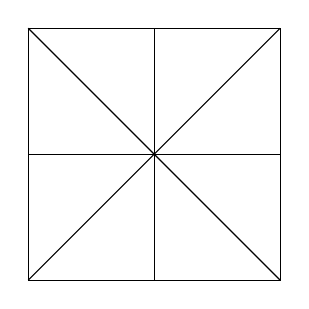
\begin{tikzpicture}[scale=0.4]
		\draw (0, 0) -- (8, 0) -- (8, 8) -- (0, 8) -- (0, 0);
		\draw (4, 0) -- (4, 8);
		\draw (0, 4) -- (8, 4);
		\draw (0, 0) -- (8, 8);
		\draw (0, 8) -- (8, 0);
		\end{tikzpicture}
		\caption{Prva subdivizija.}
	\end{subfigure}
	%\vspace[20pt]
% ####################   Druga subdivizija    ####################
	\begin{subfigure}[b]{0.4\linewidth}
		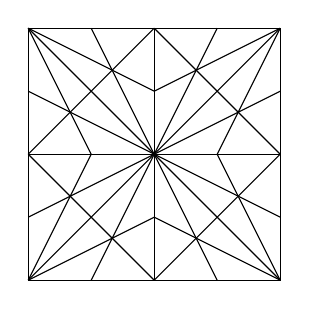
\begin{tikzpicture}[scale=0.4]
		\draw (0, 0) -- (8, 0) -- (8, 8) -- (0, 8) -- (0, 0);
		\draw (4, 0) -- (4, 8);
		\draw (0, 4) -- (8, 4);
		\draw (0, 0) -- (8, 8);
		\draw (0, 8) -- (8, 0);
		
		\subdiv{(0, 0)}{(4, 0)}{(4, 4)}
		\subdiv{(0, 0)}{(0, 4)}{(4, 4)}
		
		\begin{scope}[xscale=-1,xshift=-8cm]
		\subdiv{(0, 0)}{(4, 0)}{(4, 4)}
		\subdiv{(0, 0)}{(0, 4)}{(4, 4)}
		\end{scope}
		
		\begin{scope}[yscale=-1,yshift=-8cm]
		\subdiv{(0, 0)}{(4, 0)}{(4, 4)}
		\subdiv{(0, 0)}{(0, 4)}{(4, 4)}
		
		\begin{scope}[xscale=-1,xshift=-8cm]
		\subdiv{(0, 0)}{(4, 0)}{(4, 4)}
		\subdiv{(0, 0)}{(0, 4)}{(4, 4)}
		\end{scope}
		\end{scope}
		\end{tikzpicture}
		\caption{Druga subdivizija.}
	\end{subfigure}
	% ####################   Tretja subdivizija    ####################
	\begin{subfigure}[b]{0.4\linewidth}
		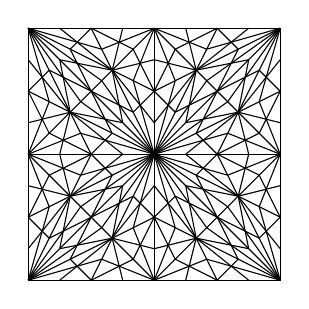
\begin{tikzpicture}[scale=0.4]
		\draw (0, 0) -- (8, 0) -- (8, 8) -- (0, 8) -- (0, 0);
		\draw (4, 0) -- (4, 8);
		\draw (0, 4) -- (8, 4);
		\draw (0, 0) -- (8, 8);
		\draw (0, 8) -- (8, 0);
		
		\subdiv{(0, 0)}{(4, 0)}{(4, 4)}
		\subdiv{(0, 0)}{(0, 4)}{(4, 4)}
		\subdiv{(0, 0)}{($(8/3, 4/3)$)}{(2, 0)}
		\subdiv{(0, 0)}{($(8/3, 4/3)$)}{(2, 2)}
		\subdiv{(0, 0)}{($(4/3, 8/3)$)}{(2, 2)}
		\subdiv{(4, 4)}{($(4/3, 8/3)$)}{(2, 2)}
		\subdiv{(0, 0)}{($(4/3, 8/3)$)}{(0, 2)}
		\subdiv{(4, 4)}{($(4/3, 8/3)$)}{(2, 4)}
		\subdiv{(0, 4)}{($(4/3, 8/3)$)}{(0, 2)}
		\subdiv{(0, 4)}{($(4/3, 8/3)$)}{(2, 4)}
		\subdiv{(4, 0)}{($(8/3, 4/3)$)}{(2, 0)}
		\subdiv{(4, 2)}{($(8/3, 4/3)$)}{(4, 0)}
		\subdiv{(4, 2)}{($(8/3, 4/3)$)}{(4, 4)}
		\subdiv{(2, 2)}{($(8/3, 4/3)$)}{(4, 4)}
		
		\begin{scope}[xscale=-1,xshift=-8cm]
		\subdiv{(0, 0)}{(4, 0)}{(4, 4)}
		\subdiv{(0, 0)}{(0, 4)}{(4, 4)}
		\subdiv{(0, 0)}{($(8/3, 4/3)$)}{(2, 0)}
		\subdiv{(0, 0)}{($(8/3, 4/3)$)}{(2, 2)}
		\subdiv{(0, 0)}{($(4/3, 8/3)$)}{(2, 2)}
		\subdiv{(4, 4)}{($(4/3, 8/3)$)}{(2, 2)}
		\subdiv{(0, 0)}{($(4/3, 8/3)$)}{(0, 2)}
		\subdiv{(4, 4)}{($(4/3, 8/3)$)}{(2, 4)}
		\subdiv{(0, 4)}{($(4/3, 8/3)$)}{(0, 2)}
		\subdiv{(0, 4)}{($(4/3, 8/3)$)}{(2, 4)}
		\subdiv{(4, 0)}{($(8/3, 4/3)$)}{(2, 0)}
		\subdiv{(4, 2)}{($(8/3, 4/3)$)}{(4, 0)}
		\subdiv{(4, 2)}{($(8/3, 4/3)$)}{(4, 4)}
		\subdiv{(2, 2)}{($(8/3, 4/3)$)}{(4, 4)}
		\end{scope}
		
		\begin{scope}[yscale=-1,yshift=-8cm]
		\subdiv{(0, 0)}{(4, 0)}{(4, 4)}
		\subdiv{(0, 0)}{(0, 4)}{(4, 4)}
		\subdiv{(0, 0)}{($(8/3, 4/3)$)}{(2, 0)}
		\subdiv{(0, 0)}{($(8/3, 4/3)$)}{(2, 2)}
		\subdiv{(0, 0)}{($(4/3, 8/3)$)}{(2, 2)}
		\subdiv{(4, 4)}{($(4/3, 8/3)$)}{(2, 2)}
		\subdiv{(0, 0)}{($(4/3, 8/3)$)}{(0, 2)}
		\subdiv{(4, 4)}{($(4/3, 8/3)$)}{(2, 4)}
		\subdiv{(0, 4)}{($(4/3, 8/3)$)}{(0, 2)}
		\subdiv{(0, 4)}{($(4/3, 8/3)$)}{(2, 4)}
		\subdiv{(4, 0)}{($(8/3, 4/3)$)}{(2, 0)}
		\subdiv{(4, 2)}{($(8/3, 4/3)$)}{(4, 0)}
		\subdiv{(4, 2)}{($(8/3, 4/3)$)}{(4, 4)}
		\subdiv{(2, 2)}{($(8/3, 4/3)$)}{(4, 4)}
		
		\begin{scope}[xscale=-1,xshift=-8cm]
		\subdiv{(0, 0)}{(4, 0)}{(4, 4)}
		\subdiv{(0, 0)}{(0, 4)}{(4, 4)}
		\subdiv{(0, 0)}{($(8/3, 4/3)$)}{(2, 0)}
		\subdiv{(0, 0)}{($(8/3, 4/3)$)}{(2, 2)}
		\subdiv{(0, 0)}{($(4/3, 8/3)$)}{(2, 2)}
		\subdiv{(4, 4)}{($(4/3, 8/3)$)}{(2, 2)}
		\subdiv{(0, 0)}{($(4/3, 8/3)$)}{(0, 2)}
		\subdiv{(4, 4)}{($(4/3, 8/3)$)}{(2, 4)}
		\subdiv{(0, 4)}{($(4/3, 8/3)$)}{(0, 2)}
		\subdiv{(0, 4)}{($(4/3, 8/3)$)}{(2, 4)}
		\subdiv{(4, 0)}{($(8/3, 4/3)$)}{(2, 0)}
		\subdiv{(4, 2)}{($(8/3, 4/3)$)}{(4, 0)}
		\subdiv{(4, 2)}{($(8/3, 4/3)$)}{(4, 4)}
		\subdiv{(2, 2)}{($(8/3, 4/3)$)}{(4, 4)}
		\end{scope}
		\end{scope}
		\end{tikzpicture}
		\caption{Tretja subdivizija.}
	\end{subfigure}
\caption{Slika prikazuje primer prve, druge in tretje subdivizije kocke $C$.}
\end{figure} 

\end{document}